\documentclass[12pt]{article}

\usepackage{txfonts}
\usepackage[T1]{fontenc}
%\usepackage[latin1]{inputenc}

\usepackage{array}
%\usepackage{lscape}
\usepackage{rotating}
\usepackage{longtable}
\usepackage{booktabs}
%
% Change coordinates to edge of page
\voffset=-1in \hoffset=-1in
%
% Set for US Letter
\textheight=9.0in \textwidth=6.5in \topmargin=0.5in
\oddsidemargin=1in \evensidemargin=1in
%
\frenchspacing \raggedbottom
%\renewcommand{\thesection}{\Alph{section}}
%\renewcommand{\theenumii}{\arabic{enumii}}
\newcommand{\tight}{\itemsep 0pt}
%\newcommand{\ve}[1]{\mathbf{#1}}
\newcommand{\vk}[1]{\mbox{\boldmath $#1$}}
\newcommand{\tabfoot}[1]{$^{\footnotesize{\textrm{#1}}}$}

\begin{document}

\title{Incorporating Land Use in\\Metropolitan Transportation Planning\\}

\author{Paul Waddell$^{\dagger}$ \and Gudmundur F. Ulfarsson$^{\triangle}$
\and Joel Franklin$^{\ddagger}$ \and John Lobb$^{\circ}$
\and\\ \\
$^{\dagger}$ Evans School of Public Affairs and
\\Department of
Urban Design and Planning,University of Washington, \\ Box 353055, Seattle, WA 98195 \\
(206) 221-4161, pwaddell@u.washington.edu \\\\
$^{\triangle}$ Department of Civil Engineering, Washington
University in St. Louis, \\ Campus Box 1130, One Brookings Drive,
St. Louis, MO 63130 \\ (314) 935-9354, gfu@wustl.edu \\\\
$^{\ddagger}$ Department of Urban Design and Planning\\ University
of Washington\\Box 355740, Seattle, WA 98195\\(206) 616-4499,
joelpf@u.washington.edu\\\\
$^{\circ}$ Resource Systems Group, Inc.\\55 Railroad Row \\ White River Junction, VT 05001\\
(802) 295-4999, JLobb@rsginc.com\\\\\\
Submitted to Transportation Research, Part A: Policy and
Practice\\\\
Revised}

\maketitle \clearpage

\abstract

In current practice, very few Metropolitan Planning Agencies
attempt to capture the effects of transportation system changes on
land use, and the consequent feedback effects on transportation
system performance, despite substantial evidence that these
effects may be significant. In this paper, we present a case study
on the application of UrbanSim, a detailed land use simulation
model system, and its integration with a regional travel demand
model in the Greater Wasatch area of Utah. Like several other
metropolitan areas, this region has recently been confronted with
legal challenges to proposed highway projects, drawing substantial
scrutiny to the land use-transportation connection.  We describe
the UrbanSim model specification, results from model estimation,
and sensitivity analyses conducted with the combined land use and
travel model system.  The results of the sensitivity analysis
suggest that accounting for the land use effects of a regional
transportation plan may produce significant shifts in key
transportation evaluation measures such as vehicle miles traveled,
vehicle hours traveled, and hours of congestion delay.

\section{Introduction}
The impact of transportation improvements on urban development is
perhaps one of the most important, and contested, concerns in
metropolitan transportation planning today.  On the one hand, it
has long been known that transportation accessibility
fundamentally influences firm location, household location, real
estate development, land prices, and density (von Th�nen, 1826;
Muth, 1969; Mills, 1967; Alonso, 1964).  The practice of
transportation planning, however, has until recently routinely
ignored the effects of major transportation improvements on urban
form, and the consequent indirect effects that such induced
development can have on the efficacy of alternative transportation
investment strategies. Regional Transportation Plans prepared by
Metropolitan Planning Organizations very rarely acknowledge any
feedback effects from transportation improvements on land use, and
thereby ignore these effects on project and plan evaluation.  This
omission has the potential consequence of exaggerating mobility
and environmental benefits of transportation projects, and
undervaluing the potential benefits of land use or integrated land
use and transportation policies.

The importance of this feedback of transportation on land use has
been recognized in federal policy since the passage of the Clean Air
Act Amendments of 1990 and the Intermodal Surface Transportation
Efficiency Act of 1991, and has prompted legal challenges by
environmental advocates in numerous metropolitan areas on the
grounds that air quality conformity results may be overly optimistic
where these feedback effects are ignored. Although some research has
argued that the relative effects of accessibility are becoming less
important in determining outcomes such as residential location as
compared to other factors such as amenities (c.f. Giuliano, 2004),
the fact remains that there is a very high degree of mutual
influence between the evolving urban form of a metropolitan area and
its transportation system. Why, then, is this effect so widely
ignored in contemporary metropolitan transportation planning?

One explanation that has been put forward is an institutional and
political one: the predisposition of transportation planning
institutions towards road construction, whereby there is an
incentive to ignore feedback effects such as long-term induced
demand that might reduce the perceived value of desired projects.
Given that much of the funding for road improvements is from
federal sources, there is a potential incentive to export the
costs of these projects and not fully account for these costs when
evaluating projects. Whether or not this hypothesis is valid, it
does not provide a compelling rationale to ignore the effects of
transportation on land use. A second explanation that has some
credibility is that there is insufficient theoretical
understanding of the interconnections between transportation and
land use, or alternatively that these connections are too complex
and chaotic to account for in a formal analysis or model.  This
explanation may have some merit, but advances in theoretical and
quantitative analysis on location choice, urban development, and
real estate markets suggests that this rationale is insufficient
to justify failing to account in some form for these feedbacks.
Finally, the claim that there are no available models for
widespread use by planning staff in Metropolitan Planning
Agencies, or that the models are too complex or data hungry, is
raised as a practical limitation. While there has been a long
hiatus in the development of land use models for integrated land
use and transportation planning, there has been a rapid resurgence
in research and development of such models over the past five to
ten years, though the assessment of these models remains sparse
(Miller, Kriger and Hunt, 1999; Dowling \emph{et al}, 2005).  This
paper addresses these barriers to incorporating
transportation-land use interaction into contemporary metropolitan
transportation planning, by describing a case study in the
operationalization of an integrated land use and transportation
model system, in the context of legal contention over a highway
project.

The objective of this paper is to present the results of a project
to evaluate the application of the recently developed UrbanSim
land use model system and its integration with the Wasatch Front
Regional Council (WFRC) four-step travel model system.  We
describe as thoroughly as available space permits the process of
developing and applying UrbanSim in the Greater Wasatch Front
Region, including the development of the database, estimation and
calibration of model parameters, integration with the WFRC travel
model system, and validation of the model system through
sensitivity analysis designed to explore the responsiveness of the
model to major transportation system and land use policy changes.
A key finding of this research is that by incorporating the
feedback of transportation on land use, predictions of the vehicle
miles traveled (VMT) and vehicle hours traveled (VHT) increase by
5\% compared to the 2030 Long Range Plan baseline (which did not
consider this feedback), and the total hours of congestion delay
(TCD) increased by almost 16\%, confirming that this feedback is
important to address in regional transportation planning.

The paper is organized as follows.  In the next section, we
describe the political and institutional context of the case
study, which presents challenges that are at least as important as
the technical ones.  We then describe the project scope, including
the evaluation framework for the project.  Following this, we
provide an overview of UrbanSim and its components, including
representative results from the model development and estimation
in this region.  We then address the coupling of UrbanSim and the
regional travel model system, followed by a discussion of
sensitivity analyses designed to test the integrated model system.
The paper concludes with discussion of the evaluation of the Peer
Review Panel, subsequent actions taken by the WFRC to bring the
integrated model system into operational use, and concluding
comments and directions for further research.

\section{Political and Institutional Context}
The Greater Wasatch Area, containing 80 percent of Utah's
population and centered on Salt Lake City, is a rapidly growing
metropolitan area.  The problems presented by Utah's rapid growth
are compounded by several factors unique to the area, including
the physical constraints imposed by the surrounding mountains and
the Great Salt Lake, and by an abundance of critical environmental
resources that require protection.  These constraints limit the
supply of developable land to accommodate a projected doubling of
the region's population and employment over the next thirty years,
precipitating an increasing sense of urgency about how to maintain
the quality of life the region enjoys, including the quality of
its natural environment.

By the year 2020, population and travel demand in the five
counties along the eastern shore of the Great Salt Lake is
predicted to increase by 60 and 69 percent, respectively. In order
to deal with this projected demand, Utah state, regional, and
local officials developed a series of transportation improvement
plans collectively known as the "Shared Solution." The Shared
Solution calls for widening Interstate 15, enhancing
transportation systems and management, increasing the availability
and usage of mass transit, and constructing the Legacy Parkway
Project.

The Legacy Parkway is planned as a four-lane, limited-access,
divided highway starting near Salt Lake City and extending north
approximately 14 miles to US 89.  The project includes a
pedestrian/equestrian/bike trail and will block traffic noise by
using earthen berms rather than sound walls.  The 14-mile Legacy
Parkway should not to be confused with the 100+-mile Legacy
Highway - running from Brigham City to Nephi - proposed by Utah
Governor Michael Leavitt in 1996.  That project has been the
subject of considerable controversy, leading to a series of legal
challenges.

In order to begin construction, the Legacy Parkway Project
required approval from the Federal Highway Administration (FHWA)
because it would merge with the interstate highway system.  The
project also needed to obtain a 404(b) permit from the U.S. Army
Corps of Engineers (COE) because construction would entail the
filling of 114 acres of wetlands. Both the FHWA approval and COE
permit were considered major federal actions that required an
Environmental Impact Statement (EIS). Between 1996 and January
2001 the Utah Department of Transportation (UDOT) prepared a draft
and final EIS, awarded the contract for construction of the Legacy
Parkway, obtained the COE 404(b) permit, and was granted approval
by the FHWA.

In response to these approvals, on January 17, 2001, the NGO
Utahns for Better Transportation (UBT) and Salt Lake City Mayor
Rocky Anderson filed a suit in federal district court alleging
that the FHWA and COE violated the National Environmental Policy
Act (NEPA) and the Clean Water Act (CWA). The Sierra Club filed a
second suit against the U.S. Department of Transportation adding a
Clean Air Act (CAA) complaint alleging that the Salt Lake area
Transportation Implementation Plan was in violation of
transportation conformity requirements and that Legacy Parkway
would result in increased mobile source emissions. The UBT and
Sierra Club cases were consolidated by the district court and the
CAA conformity claims were separated from the Legacy Parkway
permitting and review claims.

On August 11, 2001, U.S. District Judge Bruce S. Jenkins dismissed
the plaintiff's permitting and review claims, upholding the 404(b)
permit decision and FHWA approval process, thereby ruling in
UDOT's favor.  The plaintiffs filed for injunctive relief with the
federal district court and after being denied, filed for
injunctive relief with the 10th Circuit Court of Appeals.  On
November 16, 2001, the 10th Circuit Court of Appeals granted
injunctive relief and construction on Legacy Parkway was halted.
On September 16, 2002, the court ruled in favor of the plaintiffs,
citing inadequacies of the EIS and the permitting process.

On June 26, 2002, the Sierra club, U.S. DOT, FHWA, Federal Transit
Administration (FTA), COE, and the State of Utah entered into an
agreement to settle the conformity claims against the Legacy
Parkway.  Under the terms of the settlement, one element
stipulated that an assessment be conducted of the use of UrbanSim
in conjunction with the regional travel model system operated by
the WFRC. A favorable assessment of UrbanSim would obligate WFRC
to begin using UrbanSim to produce socioeconomic and development
forecasts and integrate these into WFRC's operational planning
activities, such as updating the Long-Range Transportation Plan
(LRP), Transportation Improvement Program (TIP), and corridor
planning projects.  This assessment was financially supported by a
grant from FHWA that had been made independently as a match to a
National Science Foundation Digital Government grant awarded to
the University of Washington.

In many ways, the controversy over this highway project reflects a
broader trend across the nation, with many metropolitan regions
facing similar problems, as highway projects have become embroiled
in political and increasingly legal battles.  The origins of the
controversies vary from place to place, but there are common
elements, such as concerns over the long-term effects of major
highway on urban development and additional travel. While not
every aspect of this particular case is generalizable to others,
it is likely that lessons learned in this case may have some
bearing on other, similar cases.  In the words of an anonymous
reviewer, "It presents a potential landmark precedent for the
requirement of alternative land use scenarios to be required in
regional long range transportation planning."

\section{Project Scope}
The assessment of the integration of UrbanSim with the regional
travel model system was launched in 2003 with the formation of a
Peer Review Panel and the organization of a Management and Policy
Committee and a Scenarios Committee.  The Management and Policy
Committee represents stakeholders from WFRC management and other
related organizations, and was established to address questions
relating to the incorporation of UrbanSim into the policy and
institutional setting in the region.  The Scenarios Committee
consists principally of planners from jurisdictions in the region,
and was established to provide local input to and review of
scenarios tested.  The Peer Review Panel, consisting of technical
experts in land use and transportation modeling, were charged with
the overall coordination of the evaluation, and with making
recommendations to the WFRC on the use of UrbanSim in operational
planning.  Due to the schedule stipulated in the terms of the
settlement, the entire review had to be completed by the end of
2003.

The first meeting of the Peer Review Panel (PRP) was held June
26-27, 2003 to organize the work scope and obtain initial feedback
from the PRP.  The core of the recommendations of the PRP were to
document the model system and its development and calibration, and
to conduct a validation of the combined UrbanSim - Travel Model
system using a series of tests, which we describe in detail in
section \ref{se:sensitivity}.

\subsection{Framing the Evaluation}
The evaluation of UrbanSim (or any other model) as a tool for
operational planning in conjunction with the regional travel models
involves many considerations, broadly grouped into the validity of
the model system and its usability. Some of the questions the
evaluation of the UrbanSim model application were intended to
consider are outlined below.  We return to the summary assessment of
these questions by the Peer Review Panel in the closing section.

\subsubsection{Model Validity}
\begin{itemize}
\item Is the model structure theoretically sound? Based on a
review of the written documentation of the model system and of the
presentations, are there any theoretical deficiencies in the model
design that would undermine the validity of the model and its
capacity to address the intended planning functions within the
region?  Are there areas in which it could be improved?

\item Are the quantitative methods used in the model appropriate?
Are there any concerns about the validity of the quantitative
methods used in the model system (multinomial logit, multiple
regression, monte carlo simulation)?

\item   Are the estimation results valid? Based on review of the
documentation of the model specification and estimation results
for the Wasatch Front region, are there any significant concerns
about the estimation results that would call into question the
validity of the model?

\item   Are the simulation results reasonable? Given the absence
of sufficient historical data with which to undertake a historical
validation of the model in the Wasatch Front Region, the
simulation results must be evaluated against theory and local
knowledge.  Based on this review, are there any significant
concerns about the validity of the simulation results?

\item Is the model appropriately sensitive to constraints and
policies of interest, especially effects of major transportation
improvements? Do the model predictions show patterns of response
to changes in key policy variables, such as the transportation
system, that are consistent with theory and local knowledge?  To
which policies should the model be made sensitive in the regional
planning context?

\item Does it integrate well with the regional travel model
system? Is the approach to integration with the travel model
specified and implemented in a way that is consistent with theory?

\end{itemize}

\subsubsection{Model Usability}
\begin{itemize}
\item Does the model have an effective user interface? What
characteristics would be useful in the user interface to support
the range of intended applications for the model?

\item Is the computing performance adequate? What level of
computing performance would define a usable system for interaction
with the travel model system, given an expectation of running the
travel model approximately every 10 years of simulated time?

\item Are requirements for data and expertise manageable? What
level of staff support and expertise is appropriate to devote to
the land use model as a part of the broader integrated regional
modeling system?  Do UrbanSim's requirements fall within those
limits?

\item Does it produce needed indicators or performance measures
for diagnosis and evaluation? Given the range of possible policies
to be evaluated, which indicators would be useful to local
stakeholders for effectively evaluating alternative policy
scenarios?

\item Does it integrate adequately into the institutional and
political context? What are the institutional and political concerns
regarding the use of UrbanSim in the region?  How should the
UrbanSim implementation be managed and accessed by various
stakeholders in the roles of creating scenarios, running the model
system, and evaluating results?  How should local land use policies,
major transportation alternatives, major development plans, regional
visioning, and other significant inputs be incorporated?

\item How useful is it in different use cases, including updating
the regional transportation plan, corridor planning, regional
visioning, and local community planning? What are the different
usage contexts, or situations, envisioned for applying UrbanSim?
In each of these use cases, who are the stakeholders and what
criteria are important to them in evaluating the use of the model
system?

\end{itemize}

\subsection{Comparison to Current Procedures} In order to assess
the potential for operational use of UrbanSim by the WFRC, it must
be examined in comparison to the existing operational procedures
for land use forecasting.  The current land use forecasting
procedure is based on a trend-based model to allocate households,
population and jobs by five sectors to Traffic Analysis Zones.  It
is implemented in a spreadsheet, and has enhancements to account
for capacity constraints and planned developments.  The land use
forecasting process relies on considerable review and adjustment
based on an expert panel and by the cities in the region.  It does
not attempt to include any assessment of feedback of
transportation improvements on land use.

\section{Overview of UrbanSim} \label{se:overview-of-model}

In this section of the paper we describe the theory and
specification of the model system and its components as applied to
the Greater Wasatch Front Region. UrbanSim is a simulation system
that integrates several land use model components, and has been
linked to a recently updated travel demand model system in Utah.
Fig. 1 depicts the model components and their relationships. The
UrbanSim model system and software architecture is described in
detail elsewhere (Waddell, 2002; Waddell et al., 2003a; Noth et
al., 2003), and is available as Open Source software at
http://www.urbansim.org.  Compared to existing operational land
use models, UrbanSim is unusual in several respects, but most
notably its use of individual agents, the explicit representation
of the demand and supply sides of the real estate market as well
as prices, a dynamic representation of time (as compared to
equilibrium models), and its design to be sensitive to a range of
policies.  A detailed comparison of UrbanSim to other models is
beyond the scope of this paper, but thorough model comparisons are
available in Miller, Kriger and Hunt, 1999 and Dowling et al.,
2005.

\subsection{Integrated Model Architecture} \label{se:architecture}

As a complete land use and transportation model system, UrbanSim
includes five interacting models, and it links to two exogenous
model systems: a macroeconomic model, to predict future
macroeconomic conditions such as population and employment by
sector; and a travel demand model system, to predict travel
conditions such as congested travel times and composite utilities of
travel between each interchange. Since the macroeconomic model does
not depend on outputs from UrbanSim, the macroeconomic data can be
forecast independently and used as fixed inputs to UrbanSim.


The main model components in UrbanSim, in the order of their
execution, are the accessibility model, the economic and
demographic transition models, the household and employment
mobility (intra-urban relocation) models, the household and
employment location choice models, the real estate development
model, and the land price model. Each of the key model components
are described in more detail in Sections \ref{se:choice-models}
through \ref{se:land-price}. Data flows among model components are
shown in Fig. \ref{fig:USStruct}.

The model system reads exogenous inputs not only from external
macroeconomic and travel demand models, but also from user input.
These user inputs include assumptions reflecting land use policies
that regulate real estate development, and any user-specified events
that describe scheduled events representing changes in employment,
real estate development or land policy the user intends to apply to
the model in a specific simulation year.

A key element of the model system is that real estate development is
acknowledged to require a longer time frame than location choices
made by firms and households. Developers must monitor market
conditions and trends, acquire a site, acquire financing, obtain
permits, prepare the site (often requiring infrastructure
extensions), and undertake construction that might require several
years in the case of large-scale projects. As a result, the
interaction of demand and supply sides of the market can be
characterized as an ongoing series of adjustments to varying degrees
of market disequilibrium. Building booms and busts, and volatile
swings in rents, prices and vacancy rates, are all well-known
symptoms of the disequilibrium in real estate markets. This
perspective leads to a model design that reflects the models of
demand as operating in a short-term period (which we simplify to
under one year), given a fixed supply of real estate within this
time frame. Choices of developers, on the other hand, are modeled as
a response to current and previous market conditions, and
development projects are scheduled for implementation at least one
year in the future to reflect the inherent time lags in the
development process. The dynamic adjustment of demand, supply and
prices used in the UrbanSim design, and the path dependence that it
generates, contrasts with the more traditional static equilibrium
modeling approach taken in other land use models that simulate real
estate markets.

\subsection{The Database} \label{se:database}

The input data used to construct the model database include parcel
files from tax assessor offices; business establishment files from
the state unemployment insurance database or from commercial
sources; census data; GIS overlays representing environmental,
political, and planning boundaries; and a location grid. A set of
software tools, collectively referred to as the data integration
tools, reads these input files, diagnoses problems in them such as
missing or miscoded data, and applies decision rules to synthesize
missing or erroneous data and construct the model database.

Each household in the metropolitan area is represented in the
database as an individual entity, with the primary characteristics
relevant to modeling location and travel behavior: household size,
number of workers, presence of children, age of head, and
household income. The household list is synthesized by integrating
census household-level data from the Public Use Microdata Sample
with Summary Tape File 3A tabulations by census tract, and
assigning synthesized households probabilistically to parcel data,
using a variant of the procedure developed for the TRANSIMS model
system (Beckman et al., 1996). Employment is represented in the
database as individual records for each job and its employment
sector.

Locations are represented using grid cells of 150 by 150 meters,
which contain an area just over 5.5 acres (the cell size can be
modified). This location grid allows explicit cross-referencing of
other spatial features including planning and political boundaries
such as city, county, traffic zones, urban growth boundaries; and
environmental features such as wetlands, floodways, stream
buffers, steep slopes, or other environmentally sensitive areas.

Parcel data are collapsed into the cells to generate composite
representations of the mix and density of real estate at each
location, which we refer to as development types. These
development types are somewhat analogous to the development
typology developed by Calthorpe (1983), in that they represent at
a local neighborhood scale the land use mix and density of
development. A database table stores the rules for classifying
grid cell development into types, based on the combination of
housing units, nonresidential square footage, and the principal
land use of the development.

The database maintains an explicit accounting of real estate and
occupants, linking individual households to individual housing
units, and individual jobs to job spaces that can be either
nonresidential square footage or a residential housing unit to
account for home-based employment. When jobs or households are
predicted to move, the space they occupy is reclassified as
vacant, and when they are assigned to a particular housing unit or
job space, that space is reclassified as occupied. By explicit
assignment of housing units and nonresidential square footage to
grid cells of fixed size, densities and mixtures of housing units
and nonresidential square footage of industrial, commercial, or
governmental types are inventoried.  Land values and residential
and nonresidential improvement values are also identified for each
cell in the database. This integrated database of households,
jobs, land, and real estate is what the model components update
over time. Although this database is derived from data about
real households, businesses, and parcels, it is a synthetic
database that represents only selected characteristics of people,
jobs, real estate, and locations. Similarly, the models and their
estimated parameters attempt to reflect the patterns of observed
behavior of real agents but are simplifications and abstractions
of real behavior, as are all models.


\subsection{Discrete Choice-Based Model Components}
\label{se:choice-models}

Exploiting the Random Utility Maximization (RUM) models pioneered
by McFadden (1974, 1981), UrbanSim implements the residential
location choice, employment location choice, and real-estate
development choice models as discrete choice models.  We describe
this common framework before discussing each model component
individually. We assume that each alternative $i$ has associated
with it a utility $U_i$ that can be separated into a systematic
part and a random part:
\begin{equation}
    U_i = u_i + \epsilon_i,
    \label{eq:utility}
\end{equation}
where $u_i = \vk{\beta}\cdot\vk{x}_i$ is a linear-in-parameters
function, $\vk{\beta}$ is a vector of $k$ estimable coefficients,
$\vk{x}_i$ is a vector of observed, exogenous, independent
alternative-specific variables that may be interacted with the
characteristics of the agent making the choice (e.g. household
characteristics in the residential location choice model), and
$\epsilon_i$ is an unobserved random term. Assuming the unobserved
term in (\ref{eq:utility}) to be distributed with a Gumbel
distribution (Type I extreme value distribution) leads to the
familiar multinomial logit model (McFadden 1974, 1981):
\begin{equation}
    P_i = \frac{\mathrm{e}^{u_i}}{\sum_j \mathrm{e}^{u_j}},
    \label{eq:mnl}
\end{equation}
where $j$ is an index over all possible alternatives. The
estimable coefficients of (\ref{eq:mnl}), $\vk{\beta}$, are
estimated with the method of maximum likelihood (see for example
Greene, 2002).

We have used standard multinomial logit specifications throughout
the model system, which have a closed form specification of the
probabilities and are efficient computationally.  More flexible
choice model specifications are available, such as mixed logit,
and may be suitable for the models at hand, but come with
considerable computational expense, since they lack closed form
probabilities.  Given the need for computational efficiency in
this project, we leave for future work the examination of
alternative discrete choice model specifications.  Similarly, one
might contend that decision-makers are not always rational, or
that they might use particular heuristics for searching or
selecting among alternatives.  While there may be merit to these
concerns, we do not resolve them in the current project.  In later
work we have begun to generalize the choice modeling framework to
allow testing of alternative choice model specifications and
heuristics.

\subsubsection{Employment Location Choice} \label{se:elc}

We begin the description of UrbanSim models with a description of
the employment location choice model, as employment location is a
critical driver of urban form. Theoretical models of employment
location date at least to the seminal work of von Th�nen (1826),
which described a negatively sloped agricultural land rent gradient
as distance from a central market increases to offset increased
transportation costs to the market. This early work on bid-rent
later stimulated the development of the monocentric model of urban
structure (Muth, 1969; Mills, 1967; Alonso, 1964). Early
applications of spatial theory of urban firm location can be traced
to Christaller's (1933) work on central place theory and the
hierarchy of cities, and that of L�sch (1944), who derived an
idealized hexagonal representation of market areas based on spatial
competition between firms. These early contributions provided
conceptual foundations for understanding the competitive bidding for
sites with higher accessibility, which produces declining land rent
gradients from high access locations, and the spatial separation of
firms competing for market share.  These frameworks, however, are
insufficient to explain widespread emergence of secondary suburban
centers and specialized employment clusters in the latter third of
the 20th century.

A critical contribution to the theory of firm location that does
address the emergence of employment clusters and centers is the
concept of agglomeration economies, which describe positive
externalities associated with spatial proximity to firms within the
same or related industries. These agglomeration economies have been
described as arising from information spillovers, local non-traded
inputs, and a local skilled labor pool (Marshall, 1920). An
important theoretical problem in urban economic models is that
neoclassical economic assumptions include constant returns to scale,
but the essence of agglomeration economies is the idea of increasing
returns to scale for firms that cluster with other firms in their
own or related industrial sectors (Krugman, 1991). There are
offsetting forces that neutralize the agglomeration advantages of
clustering as centers become large, producing opportunities for the
creation and growth of suburban centers. Other relevant work on
employment location has focused on transportation costs (Chinitz,
1960), the influence of amenities and governmental services and
taxes (Bartik, 1991; Waddell and Shukla, 1993).

The employment location choice model in UrbanSim draws on these
antecedents, bringing together the concepts of bid-rent theory,
agglomeration economies, and the effects of transportation and
local government policy in a discrete choice model. The model
simulates location choices for new jobs created as a byproduct of
economic expansion, predicted by an external macroeconomic model,
and for jobs that have been predicted to move by the employment
relocation model component of UrbanSim. To arrive at a choice
model for employment location we assume that 1) each job belongs
to a firm (whose characteristics other than industry sector remain
latent) which is faced with a choice between alternative locations
for the job, 2) that each location, indexed by $i$, has attached
to it some utility, $U_i$, for the firm, and 3) that the location
with the highest utility has been chosen (maximization of
utility).

We refer to the more general concept of utility maximization rather
than profit maximization, since the utility may be based largely or
exclusively on expectations of profit for some sectors, but profit
may represent a small or nonexistent part of the utility for other
sectors, such as governmental and educational establishments. In the
date we use for model estimation, we only observe the current
location of jobs, and do not observe the alternative locations open
to the employer before locating the job, nor do we observe the
utility. We proceed with the multinomial logit assumptions for the
utility (\ref{eq:utility}) leading to (\ref{eq:mnl}).

The systematic component of the utility of a particular location
(dropping the index $i$ for simplicity in this and subsequent
equations) is specified as a function of an array of
characteristics at the \emph{site} ($\vk{x}_S$), including the
real estate characteristics (land value, residential units,
commercial sq. ft., land use) and proximity of the site to
freeways and arterials; characteristics of the land use mix and
value (quantity of residential units, average land values, average
improvement values) in the immediate \emph{neighborhood}
surrounding the site ($\vk{x}_N$); agglomeration economies from
geographic \emph{clustering} (employment by sector within 600 m)
of firms of the same and each of the other sectors ($\vk{x}_C$);
and multi-modal \emph{accessibility} to labor, consumers, the
Central Business District (CBD), and the regional airport
($\vk{x}_A$):
\begin{equation}
    u = \vk{\beta}_S \vk{x}_S
     + \vk{\beta}_N \vk{x}_N
     + \vk{\beta}_C \vk{x}_C
     + \vk{\beta}_A \vk{x}_A.
     \label{eq:uemploc}
\end{equation}

The probability, $P_i$, represents the probability of the firm
choosing location alternative $i$ for a particular job. We
estimate one choice model (i.e. one set of coefficients) for each
of the 14 industry sectors shown in Table~\ref{ta:sectors} on a
random sample of 5000 observed jobs in each sector. To estimate
the model coefficients we use data for business establishments in
1997, geo-coded to grid cells. The database links individual jobs
to job spaces. The job spaces can be either nonresidential square
footage, or a residential housing unit to account for home-based
employment.

To arrive at a set of alternatives we allow each job in a sector to
consider as alternatives all locations feasible to that industry
sector. This generates a choice set containing potentially hundreds
of thousands of alternatives, which would be intractable to estimate
a choice model with. We use a uniform distribution to randomly
sample a set of nine alternatives in addition to the chosen location
and estimate a model using this random sample of alternatives.  It
has been shown previously that the coefficients of a choice model
estimated from a random sample of alternatives, selected with a
uniform distribution, are consistent, as explained by McFadden
(1978) in his paper on residential location choice, which addressed
a similar issue (see also Train, 2003).

Since the coefficients are based on random sampling of alternatives,
there are no alternative-specific constants, and no base
alternative. The coefficients are therefore interpretable in terms
of the direction of the influence of a variable on the utility and
the probability of a location choice. In addition, coefficients can
be compared across industry sectors, since the same specification is
used for all sectors, with the exception of insignificant variables,
which were restricted to zero. Estimation results for sectors 6-10
are given in Table \ref{ta:emp6-10}, for purposes of illustrating
thew model specification and types of variables considered. Full
results for all sectors are documented in Waddell \emph{et al}
(2003b).

\subsubsection{Residential Location Choice} \label{se:rlc}

The model of residential location closely mirrors the preceding
description of employment location choice, and as it has been
described previously in the literature (Waddell, 2000; Waddell and
Nourzad, 2002), we abbreviate its description here. The residential
location choice model predicts the probability that a household will
select a location, specified by a grid cell of 150 by 150 meters.
Each grid cell can include zero or more housing units and households
can only select cells with vacant housing. All housing units on a
cell are assumed to be identical and we therefore do not assign the
household to a particular unit.

Like the employment location choice model, this is a disaggregate
choice model at the grid cell level, representing over 500,000
housing units over approximately 150,000 cells. As before, we use
random sampling of alternatives for model estimation.

As before, the model is specified as a multinomial logit model
(\ref{eq:mnl}) with a systematic utility for a particular location
on the form:
\begin{equation}
    u =  \alpha
     + \vk{\beta}_H \vk{x}_H
     + \vk{\beta}_R \vk{x}_R
     + \vk{\beta}_N \vk{x}_N,
    \label{eq:uresloc}
\end{equation}
where each utility term is a linear combination of variables that
have been grouped in to categories: $H$ indicates housing
characteristics (e.g. prices, density, age), $R$ indicates
regional accessibility, and $N$ reflects neighborhood-scale
effects (socioeconomic composition, land use mix, density, local
accessibility).

The principal data used in the analysis is based on a travel
survey conducted in the Wasatch Front region in 1997 of approximately
4,000 households. This data is supplemented with housing and
neighborhood information by linking the survey coordinates to the
UrbanSim grid cells and retrieving grid cell values for the
characteristics of housing, neighborhood, and regional access
based on the traffic analysis zone containing the cell. The
variables are drawn from the literature in urban economics, urban
geography, and urban sociology.

The model generalizes the classical urban economic trade-off between
transportation and land cost (Muth, 1969; Mills, 1967; Alonso, 1964)
by including regional and local access measures, such as those of
travel time to the classic monocentric CBD, travel time to airport,
distance to highway, multi-modal access to employment opportunities,
and local shopping. All independent variables are endogenous to the
model system---that is, they are predicted by other parts of the
model system shown in Fig.~\ref{fig:USStruct}, and therefore,
predicted values are provided in future years for the application of
the model system over periods of 30 years.

The specific variables used in the Wasatch Front model were revised
based on initial testing of the integrated model, which indicated
that the model needed to be more sensitive to budget constraints and
to the interaction between the characteristics of the locating
household and the socioeconomic composition of the neighborhood
under consideration.  The specification of the household location
choice model includes variables representing the interaction of
household characteristics and the characteristics of residential
locations. Descriptive names for variables are included in the
presentation of the results below. The variables used in the
residential model estimation and the results of the model estimation
are presented in Table~\ref{ta:hou}.

\subsubsection{Real-Estate Development} \label{se:dev}

The real estate development model implements the supply side of the
model system to interact with the two preceding demand models of
employment and household location choice as well as the land price
model. Real estate development occurs as a collection of choices and
actions taken by individual developers on individual sites regarding
whether and how to develop or redevelop those sites. We assume their
behavior is motivated by profit expectations, within constraints
imposed by their resources, the physical environment, and by public
land use regulations such as local comprehensive plans and
protection of environmentally sensitive areas. The main influences
on development choices are factors influencing prices of different
types of real estate at different locations, the costs of producing
those development projects, and the constraints relevant at those
sites.

There are two general approaches that developers consider in making
development choices. The first is known as the use looking for a
site, and corresponds to a specialized developer who has a specific
project in mind, and attempts to find the most profitable site for
the project. The second general approach is known as the site
looking for a use, and corresponds more closely to the landowner's
problem of sorting out which type of development construct on a
specific site, that will generate the highest return (sometimes
referred to as the `highest and best use' of the site by the real
estate industry. In the real world, both approaches occur. We have
structured the current model as a discrete choice model from the
perspective of the site looking for a use-the landowner's
perspective. This approach lends itself to formulation as a standard
multinomial logit model, where an individual landowner considers
alternative uses, or developments, for a particular site.  In
subsequent research, not reported in this paper, we have implemented
a development model from the alternative perspective of a use
looking for a site, using the same framework outlined for the
household and employment location choice models.

The purpose of the real estate development model is to simulate
discrete developer choices about whether to initiate a development
project at particular sites within a given year, what type of
construction to undertake, and the quantity of construction. The
construction of real estate can be either new development (sometimes
referred to as greenfield development) or the intensification or
conversion of existing development (referred to as infill and
redevelopment, respectively).

The probability of each alternative (no development, increasing
density of current cell within the current development type, and
transitions to other development types) being chosen is calculated
using a multinomial logit model. Similar approaches have been
developed to model land cover change (Turner and Gardner, 1991) and
land use change (Landis and Zhang, 1998), although none of these
models interact with disaggregate demand-side models of residential
and employment location choice as is done in UrbanSim.

To arrive at a choice model for development we assume that 1) each
cell has a developer agent, 2) each development alternative, indexed
by $i$, has attached to it some utility, $U_i$, for the developer,
based principally on profit expectations, and 3) the development
event with the highest utility has occurred (maximization of
utility).

To form the estimation data we take all the development event
cells, i.e. cells with a known development event and look up the
values for a set of independent variables from the grid cell
database. The independent variables in the real estate development
model include characteristics of the \emph{site} ($\vk{x}_S$),
including current development, land use plan, environmental
constraints, policy constraints, land and improvement value,
proximity to highways, arterials, existing development, and recent
development; characteristics of the land use mix, property values,
and local accessibility measures in the \emph{neighborhood}
surrounding the site ($\vk{x}_N$); and multi-modal
\emph{accessibility} ($\vk{x}_A$), including access to population
and employment and travel time to the central business district
and airport:
%
\begin{equation}
    u = \alpha
     + \vk{\beta}_S \vk{x}_S
     + \vk{\beta}_N \vk{x}_N
     + \vk{\beta}_A \vk{x}_A.
     \label{eq:developer}
\end{equation}
%
We proceed with the multinomial logit assumptions for the utility
(\ref{eq:utility}) leading to (\ref{eq:mnl}). The probability,
$P_i$, represents the probability of a developer agent for a
particular cell choosing development alternative $i$.

We now need to take into account the much larger set of cells that
didn't experience a development event. We take a random sample of
these cells to generate a set of similar size as the development
event set. This gives us a choice-based sample of cells.
Choice-based sampling only biases the alternative-specific
constants but other coefficients remain consistent (Manski and
McFadden, 1981). We adjust the alternative-specific constants
after estimation to account for this bias.

We estimate one choice model (i.e. one set of coefficients) for
each development type, since the types are very different and the
development alternatives open to each development type vary. To
estimate the model coefficients we need data for cells
experiencing no development and for cells with development events
of all types.

The estimation data are derived from the parcel and grid data for
a base year of 1997. The year-built values of the existing
development in the assessor's records are the foundations of the
process. Year-built values are imputed for records for which they
are missing by examining the surrounding cells of the same type
and drawing from the distribution of observed values. Historical
development 'events' are identified in the data for a
user-specified period of time. Events, within this framework, are
any changes in the real estate development within a cell that is
identified by examining the year built values within the data.

The procedure is capable of identifying any new construction that
has a year-built occurring within the specified time frame.
However, the procedure does not identify events that involve the
demolition of buildings at some time in the past, since normally
there is no record of demolitions within the current assessor
database. This procedure could be augmented with data derived from
building demolition and permit records.

The result is a set of cells experiencing development events that
represent all observed transitions between any pairs of development
types, including increases in density that didn't result in a
development type change, within each year of the specified
historical time frame. The time slice for determining the existence
of an event is annual, since this is the limit of the information on
the vintage of real estate. For further explanations of this
process, see (Waddell et al., 2003a). The real estate development
model is estimated separately for cells of each development type,
representing a total of 24 models. Variables used and estimation
results are given in Table \ref{ta:dev5} for Development Type 5,
reflecting cells that are initially developed in moderate density
residential use.  The estimation results for all development types
are available in Waddell \emph{et al} (2003b).

\subsection{Land Price} \label{se:land-price}

Land prices represent the interaction between demand and supply
sides of the model system, with prices fluctuating in response to
short-term (intra-year) shifts in demand and long-term
(inter-year) shifts in supply, and work in the traditional
economic sense to ration scarce supply of land and clear the
market in the short term. The theoretical foundations of the model
of land price described here draw on bid-rent theory of land
markets (Alonso, 1964; Wheaton, 1977), and on hedonic price theory
(Rosen, 1974). Our approach in modeling real estate prices assumes
that individual consumers and suppliers are too small in scale to
manipulate prices directly, making them exogenous to these
individual actors. Whereas this assumption could be argued in the
event of oligopolistic behavior by large-scale developers or large
corporations seeking sites, it is a relatively weak assumption to
impose and avoids complications arising from modeling prices as
endogenous to the interaction between consumers and sellers, such
as having to simulate search and auction processes, imperfect
information, and oligopolistic market behavior. A second
assumption is that the advantages of location, such as
neighborhood amenities and accessibility, are capitalized into
land values. This assumption follows from a wide consensus of
theoretical and empirical work in urban economics that has
consistently found that in competitive land markets, the
quasi-unique characteristic of land (they aren't producing any
more of it, every location is unique, and housing or commercial
buildings are tied to their location) implies that consumers bid
for location based on their willingness to pay for locational
attributes, and the highest bidder wins the use of the site and
sets the market price for it (Alonso, 1964; Mills, 1967).

Rosen (1974) developed the approach of hedonic price analysis,
which attempts to disentangle the implicit prices for the
components of the bundle of services provided by housing (the same
theory applies to nonresidential space). By regressing the sale
price of housing on characteristics of the housing structure and
location, we obtain estimates of the implicit prices of individual
characteristics-holding other characteristics constant-despite us
observing only the single price of the bundle for any individual
property. These implicit prices do not, strictly speaking,
represent either demand functions (willingness to pay) or supply
functions (reservation prices), but rather, the composite of all
of the willingness to pay and reservation price functions of all
consumers and sellers in the market. Given our assumption that
prices are exogenous to individual consumers or sellers, this
provides a reasonable way to estimate the land price function
within a given market.

Following DiPasquale and Wheaton (1996), we interpret market
prices of land within a metropolitan market as consisting of two
parts. The first component is a mean price level, which fluctuates
around long-term trends that are driven by short-term imbalances
between supply and demand of real estate, by interest rates and
other development costs, and in the longer-term by overall
expansion and contraction of the metropolitan economy, population,
and changes in income. The second component is the relative price
of land across sites within the metropolitan market. These
relative prices are based on relative advantage and abundance of
sites with characteristics that are valued or avoided by
consumers. As these underlying characteristics and the resulting
relative advantage change, so to do relative prices, as these
advantages are capitalized into land values. This paper focuses
principally on the characteristics influencing relative prices,
since these will have the greatest influence on intra-metropolitan
variation in real estate development and consumer location
choices.

The land value for each cell, taken as the aggregation of the land
value of the parcel fragments that lie within the cell, and
originating from the tax assessor's estimates of the land value of
each parcel, is used as the basis for the dependent variable of
the land price model. The independent variables used as
predictors-essentially the same as for the real estate development
model-are the characteristics of the cell, its surrounding
environment, and its accessibility. A semi-log specification is
used, with the log of land price as the dependent variable, as is
common in hedonic price studies since it generally provides a more
robust specification.

The model is a linear multiple-regression of the log of land
prices, $\ln(v)$, for each cell on an array of housing structural
($\vk{x}_{S}$), neighborhood ($\vk{x}_{N}$), and accessibility
($\vk{x}_{A}$) characteristics:
\begin{equation}
    \ln(v_i) = \alpha
        + \vk{\beta_S}\vk{x_{S}}
        + \vk{\beta_N}\vk{x_{N}}
        + \vk{\beta_A}\vk{x_{A}}
        + \epsilon,
\end{equation}
where $\alpha$ is the estimable intercept term; $\vk{\beta_S}$,
$\vk{\beta_N}$, and $\vk{\beta_A}$ are the estimable coefficient
vectors on the housing structural, neighborhood, and accessibility
characteristics, respectively; $\epsilon$ is an unobserved error
term, assumed to be normally distributed with mean zero and
variance $\sigma^2$.

The full set of grid cells in the study area is used in model
estimation, using base year (1997) characteristics and values. As
such, this is a cross-sectional estimation of the market hedonic
price function, rather than an estimation of a dynamic price
function. Dynamics are introduced through the process of annual
changes in the characteristics of grid cells due to simulated
results from the real estate development, residential location and
employment location models, and the external transportation model
system, all of which combine to change the characteristics of grid
cells on an annual basis.

Results of the land price model show that the model explains
approximately 75\% of the variation in the log of land value of
cells. In these results, the coefficients reported are all
significant at the 95\% level, and the coefficients are directly
interpretable. The coefficients on the continuous independent
variables that are nominal show the percentage effect on land
value in a cell associated with a one-unit change in the
independent variable (multiply the coefficient with 100 to arrive
at the percentage change). Coefficients on variables that are
log-transformed are directly interpretable as elasticities. The
interpretation of the coefficient $\beta$ on a dummy variable X in
a semi-log regression where the dependent variable is of the form
$\ln(Y)$ is that the relative effect of X on Y is given by
$\exp(\beta)-1$, and the percentage effect is 100 $\cdot
\{exp(\beta)-1\}$ (see Halvorsen and Palmquist, 1980 for details).
As usual, each coefficient must be interpreted holding all other
variables constant.  The variables used and estimation results are
shown in Table \ref{ta:lan}.

\section{UrbanSim-Travel Model Integration}
\label{se:integration}

\subsection{Regional Accessibility}

Accessibility is important for residential and employment location
choice, as well as real-estate development, and links land use and
transportation systems. As specified in the Utah model
application, separate accessibility measures are computed for each
zone of origin to jobs and to population. These measures use a
composite disutility of travel computed by the travel model mode
choice component (after iteration within the travel model system
to account for congestion effects).  Access to a specific type of
opportunity for a given origin is computed as the distribution of
opportunities at each destination weighted by the composite
utility of all modes of travel to those destinations, where the
composite utility is defined as the logsum from the mode choice
model for each origin-destination pair for a given auto-ownership
category $a$. In other words, the accessibility to jobs for a
particular residence zone increases as a function of the number of
jobs at each destination and the ease of travelling to them.  The
resulting access measure $A_{ai}$ for each location $i$ becomes:
\begin{equation}
    A_{ai} = \sum_j^J D_j\mathrm{e}^{L_{aij}},
    \label{eq:regacc}
\end{equation}
where $D_j$ is the quantity of activity in location $j$ (it is
either the population or employment depending on if we seek the
accessibility to population or employment), $L_{aij}$ is composite
utility, or logsum, for vehicle ownership category $a$, from
location $i$ to $j$, scaled to a maximum value of 0 for the
highest utility interchange to avoid exaggerating the effects of
outlier logsum values predicted by the travel model to have
positive values.

This accessibility measure has some advantages worth noting for
use in measuring land use effects of transportation in a policy
evaluation context.  First, it is broadly consistent with utility
theory and the evaluation of consumer surplus, by using the
composite utility from the mode choice logit model.  Second, it
allows the representation of benefits from improvements to
multiple modes, and from changes in all aspects of the
transportation system that have been reflected in the
specification of the travel model, such as fares, wait times, and
transfer penalties.  On the other hand, it is also limited by the
design and specification of the travel models, including the
fairly coarse representation of networks and zones, and the
consequent limitations of these models in measuring the utility
and frequency of non-motorized travel.

\subsection{WFRC Travel Model System}

The travel model system for the Wasatch Front region used in this
project was based on an integration of the models from the WFRC
and Mountainlands Association of Governments (MAG) MPO planning
areas, and extensions to incorporate non-motorized modes. The
home-based work (HBW) mode choice model is stratified by auto
ownership category. As a result, composite utilities, or logsum
values, were computed by auto ownership level for households with
zero, one, and two or more cars. The HBW nested logit mode choice
model allocates work and work-related person trips, outcome of HBW
Trip Distribution model, between motorized and non-motorized modes
and their respective sub-modes. The model addresses the following
modes:

\begin{itemize}
\tight \item{Drive Alone (single-occupant auto trips)}
\item{Shared Ride 2 (double-occupancy auto trips)} \item{Shared
Ride 3+ (auto trips with three or more occupants)}
\item{Transit-Walk to Local Bus} \item{Transit - Walk to Express
Bus} \item{Transit - Walk to Light Rail} \item{Transit - Walk to
Commuter Rail} \item{Transit - Drive to Local Bus} \item{Transit -
Drive to Express Bus} \item{Transit - Drive to Light Rail}
\item{Transit - Drive to Commuter Rail} \item{Walk-only trips}
\item{Bicycle trips}
\end{itemize}

\subsection{Coupling UrbanSim and WFRC Travel Models}

The travel demand model system must be run iteratively with
UrbanSim. The interfacing of four-step travel models with UrbanSim
could be done for each simulation year, since UrbanSim runs
annually, but the logistical difficulties presented by the
development of annual networks and running the travel model every
year would be excessive\footnote{Each run of the travel model
required 2 hours to complete on a standard desktop computer with a
Pentium 4 CPU running at 2.6 GHz. UrbanSim required approximately
one half hour per year.}. There is also not a compelling argument
to require such frequent interactions, considering that the
accessibilities in UrbanSim are updated annually to reflect
changes in the spatial distribution of population and employment.
The precipitating factors for scheduling travel model runs would
seem to be of two types: 1) any significant change to
transportation supply, such as new or modified facilities, level
of transit service, or altered prices; or 2) cumulative congestion
effects that occur due to growth and spatial distribution of jobs
and population.  In order to provide adequate feedback from
congestion effects and to reflect major supply changes, UrbanSim
and the travel models were interfaced periodically, with the
intervals being no longer than 5 years. The specific interaction
years used in this analysis were 1997 (Base Year), 2000, 2003,
2008, 2012, 2016, 2020, 2025, and 2030.

The logistics of connecting UrbanSim and the regional travel
model, which is implemented in TP+ (Citilabs), involved creating a
series of scripts to automate the extraction of data from the
UrbanSim output database, reformatting of these data to the form
required for Trip Generation in TP+, execution of the travel
model, extraction of logsums and travel times from the travel
model and inserting them into the UrbanSim scenario database, and
then running UrbanSim for the time interval until the next
scheduled travel model run.  This process was completely automated
by a script that runs UrbanSim from the base year of 1997 to the
end year of 2030, interfacing with the travel model for each of
the 8 scheduled years listed above.  The run time from start to
finish for the combined model system for a single scenario using a
standard desktop computer is under 48 hours.

\subsection{Local Accessibility}

The measures of accessibility outlined above are limited in
several respects.  First, the measurement of accessibility depends
on the travel model system, which is based on zones designed for
traffic loading, and is rather coarse to represent non-motorized
travel.  Second, the measures of accessibility do not distinguish
accessibility by personal characteristics.  We attempt to overcome
the latter problem by interacting the accessibility measures by
auto ownership with the auto ownership of the household making
location choices.  We attempt to address the limitations of zonal
aggregation in travel models by developing more localized measures
within UrbanSim.

A broad treatment of the alternative measures of local
accessibility can be found in the literature, and lies beyond the
scope of the current paper (c.f. Crane, 2000; Ewing and Cervero,
2001). The maximum distance that people in general will walk for
daily activities (e.g. grocery shopping, restaurant) is not well
defined and there is no consensus in the literature about what
measure should be used for planning purposes, but the range
reported in various studies is from approximately one-quarter to
one-half mile. This clearly depends on local conditions such as
weather, terrain, street and sidewalk configuration, and safety,
in addition to personal characteristics such as age and health
status (Waddell and Nourzad, 2002). In this study, we define the
neighborhood scale as a radius of 600 meters, which is roughly one
third of a mile. This radius is used in the spatial queries of the
area surrounding grid cells, and we measure land use and quantity
of employment by sector using this radius.

\section{Sensitivity Analysis} \label{se:sensitivity}

Based on discussion at the first Peer Review Meeting in June,
2003, a validation process was devised for this project.  Lack of
historical data precluded a historical validation exercise, as has
been done for previous UrbanSim applications (Waddell, 2002). The
process carried out in this project involved testing UrbanSim in
combination with the regional travel model system on a set of
scenarios that would allow exploration of the sensitivity of the
model system to specified changes in policy.  Note that the
exercise was not designed to evaluate the effectiveness of these
policies, but to assess the model system responsiveness to the
policies. Given the objectives of the project, scenarios were
selected that would provide valuable information about the
sensitivity of the model system that could be used to learn more
about its utility for operational planning. For ease of
interpretation, the scenarios are controlled experiments, which is
to say, only one significant input is changed in each one.
The scenarios examined were the following, shown also on the map in
Figure \ref{fig:projects}:

\begin{itemize}
\item The currently adopted WFRC {\em Long Range Plan}, phased in
over 1997 to 2030. This scenario served as a baseline to which other
scenarios were compared.

\item A {\em No-build} scenario that holds the
transportation system constant from 1997 to 2030, but includes
congestion effects. This scenario represented a typical ``no-build''
policy scenario.

\item A {\em Highway Alternative} that removes
a major section of Bangerter Highway in southern Utah County. This
scenario was intended to test the effects of remove a localized,
auto-oriented project.

\item A {\em Transit Alternative} that removes the proposed
Mid-Jordan LRT line (planned for the next 10 years, first LRP
phase). This scenario tested the removal of a localized transit
project.

\item A {\em Parking Cost Alternative} that doubles the
cost of parking in Salt Lake City. This scenario was intended to
test the sensitivity of results to cost considerations.

\item An {\em Urban Growth
Boundary Alternative} that imposes a boundary limiting urban
expansion. This scenario tested the effects of development
constraints that would come with the designation of an urban growth
boundary.

\item Two {\em Vacancy Sensitivity Tests} on
alternative values of a vacancy rate coefficient in the land price
model.  This was requested by the Peer Review Panel to examine the
model's sensitivity to vacancy rates.

\item A set of runs to
examine the effects of {\em Random Variation} in results, using
the same inputs and allowing random seeds to vary between the
runs.
\end{itemize}

Due to space limitations, only illustrative results are presented
here, focusing on the results related to transportation evaluation
measures. Detailed results for all the tested scenarios are
documented in a final report on the project (Waddell \emph{et al},
2003b). One consideration to be kept in mind when reviewing these
results is that the UrbanSim outputs include no adjustments or
`K-factors' as are generally used in other land use or travel
models. They are the direct results of input assumptions, data,
model specifications, and estimation. The previously adopted 2030
land use forecast against which the UrbanSim LRP scenario results
were compared, by contrast, had been substantially revised from
the direct results of the current WFRC land use algorithms based
on local knowledge and negotiation.

The first integrated scenario combining UrbanSim and the regional
travel model is based on the adopted Long Range Plan (LRP).
Transportation improvements are phased in within the travel model
run that immediately follows the actual year of opening of the
facility. The improvements included in the Long Range Plan are
shown in Figure \ref{fig:LRPMap}. In all the scenarios examined,
there were several common assumptions, allowing direct analysis of
the sensitivity of the model system to a specified change in
assumptions between scenarios. The common assumptions included the
total population and employment in the region in each year, the
model coefficients, land use plan assumptions, and all other
aspects of the input data except as noted in the description of
each alternative below.

In developing the input assumptions for the model, a set of
development constraints are coded to reflect the interpretation of
the Land Use Plan designations applied to each location.  These
represent the user's view of what kinds of development would be
consistent with the Land Use Plan, and these constraints play a
significant role in constraining the behavior in the real estate
development model, essentially ruling out any development outcomes
that would be inconsistent with these constraints. Among the
scenarios we tested, only the Urban Growth Boundary scenario alters
these constraints, by reducing development capacity outside the
boundary.  The development constraints, which are assumptions input
to the model by the user as part of a scenario, have a prominent
impact on the results. The assumptions made for the sensitivity
analysis on which we report need further review and refinement
before production use of the model. In particular, the residential
development constraints need some refinement to better match master
plans, and non-residential intensification in the existing built-up
areas appears overly constrained.  These are input assumptions that
are relatively easy to revise.

Each of the scenarios was simulated using the integrated model
system, with UrbanSim running every year and the travel model
running in each of the years listed in Section \ref{se:integration}.
By the end of the simulation, in the 2030 analysis year, UrbanSim
produced for each scenario a new geographic distribution of
residential units, population, workplaces, and employment, and the
geographic distributions for each of the alternatives can be
compared to the LRP scenario. To illustrate, Figures
\ref{fig:households} shows some of the Year 2030 results of the
model for the No-Build scenario, with the number of households per
grid cell in the UGB scenario compared to the LRP scenario for 2030.
Note that the households are more concentrated within the Urban
Growth Boundary, contributing to the modified travel patterns shown
in the UGB scenario.

%Here, we see a clear pattern of reduced accessibility
%across the region, with stronger effects in the outlying areas that
%would more strongly benefit from the LRP's projects. The
%accessibilities affect the behaviors in several ways, one of which
%is in the market valuation of land, which we see in Figure
%\ref{fig:AB-land-price}. A similar spatial pattern is shown here,
%but with reduced strength, since we expect land price to also be
%dependent on other factors besides accessibility. The
%accessibilities and land prices together affect the construction of
%housing units, shown in Figure \ref{fig:AB-res-units}, and again we
%see a reduction in activity in outlying areas, but the effect is
%muted due to other factors remaining constant. Also, we would expect
%the housing units that were located in those outlying areas in the
%LRP scenario would still be built, but in locations closer to the
%existing developed areas; indeed this pattern emerges in Figure
%\ref{fig:AB-res-units}. Similar results were produced for the other
%scenarios, as well as for population, workplace floor area, and
%employment across all scenarios. For each scenario, the final 2030
%population and employment levels by TAZ were passed from UrbanSim to
%the travel model for one last run under 2030 conditions.

After running the 2030 travel model for each of the alternative
scenarios tested, the results were compared using several measures
of transportation performance, shown in Table \ref{ta:travel}.  Some
key results warrant highlighting. First, perhaps the most important
element of these results is the comparison of the Long Range Plan
(LRP) scenario using UrbanSim coupled to the regional travel models,
to the previously adopted 2030 forecast, which was based on the same
transportation system assumptions, but did not account for land use
feedback effects. Accounting for these effects in the LRP scenario
resulted in more than 5\% higher Vehicle Miles Travelled (VMT) and
Vehicle Hours Travelled (VHT) than the adopted forecast for 2030.
Moreover, the Total Congestion Delay (TDC) increased by almost 16\%
compared to the adopted forecast.  These effects are quite
significant in magnitude, and confirm that the long-term induced
demand reflected in the circular relationship between travel and
urban development and location of activities significantly alters
the evaluation of transportation system plans at a regional scale.
The effects on transit mode share are relatively modest, with a
slight decline in transit mode share compared to the adopted
forecast. Unfortunately, these comparisons are partially confounded
by slightly different control totals used in the adopted forecast,
so these differences may be partially attributable to differences in
those assumptions. The remaining comparisons to the LRP scenario use
identical control totals for population and employment and are not
subject to this concern.

The remaining scenarios are all compared to a reference case of
the LRP scenario.  The pattern of results for these scenarios are
generally plausible in magnitude and direction, including the
dramatic effects of a No-Build test in which the region doubles in
population and employment but no transportation system
improvements are made over the three-decade period.  The No-Build
scenario produces a 10\% reduction in VMT compared to the LRP
scenario, a 40\% increase in VHT, an unimaginable 256\% increase
in hours of congestion delay, and a 2.3\% decline in transit mode
share.

Dropping selected highway projects in a rapidly growing section of
Southwest Salt Lake County produces a modest -0.7\% decline in VMT
and VHT, as would be expected due to the induced travel effects.
An interesting result was that this scenario produced a slightly
larger 2.3\% decline in congestion delay compared to the LRP
scenario, suggesting that the location of these highway projects
might actually induce more congestion due to the combined effects
on land use development and travel than would be the case if they
were not built.  The removal of the highway project has almost no
impact on the transit mode share. By contrast, the Transit
scenario that reflects the omission of a light rail segment in
Southwest Salt Lake County produces modest increases in VMT
(0.2\%) and VHT (0.5\%), and a more significant increase in
congestion delay (1.9\%) compared to the LRP scenario. Elimination
of this transit project produced a small reduction of 0.2\% in the
transit mode share.

The increased parking cost scenario generated 0.3\% less VMT and
0.5\% less VHT than the LRP scenario, along with a 0.9\% reduction
in congestion delay and an increase in transit mode share of
0.2\%. Finally, the imposition of an Urban Growth Boundary (UGB)
produced fairly substantial reductions of 3.3\% in VMT, 2.3\% in
VHT, and 3.0\% in congestion delay.  Transit mode share increased
by 0.2\% in this scenario, compared to the LRP scenario.

These transportation effects comprise the combined effects of the
land use and travel model integration, and demonstrate the
sensitivity of important transportation evaluation measures to the
effects of a range of changes in the transportation system and
land use policies.  Some of these changes were very large-scale,
such as the No-Build and UGB scenarios, and these had generally
clear and large effects on both land use and travel measures.  The
other scenarios were generally project-scale and much smaller in
magnitude, and as would be expected, the effects were much smaller
and in the expected the direction.


\section{Assessment by Peer Review Panel} \label{se:peer-review-report}

Upon completion of the sensitivity analysis described above, an
independent assessment of this project was prepared by the Peer
Review Panel. The following are excerpts from the final report of
the panel (Schofer, et al, 2004):

Resource requirements - data and expertise:
\begin{quote}
``UrbanSim is a new, complex modeling tool that demands better and
different data, and considerable technical expertise for
calibration and application. Additional resources in these forms
are needed to support UrbanSim use in the long term. These
resources applied to this modeling tool - and its successors -
will bring better information to support regional policy choices.
The panel encourages WFRC and its collaborators to provide these
essential resources because the information increment to be gained
in return is well worth the investment.''

``The WFRC, in collaboration with developers at the University of
Washington, has demonstrated the technical ability to calibrate
the modeling system and conduct validation tests. The panel is
concerned that the in-house WFRC modeling and database development
capabilities are stretched thin, and there appears to be little
modeling expertise at the management level to direct and sustain
this effort. The implementation and effective use of UrbanSim (or
other integrated land use transportation models) requires an
on-going commitment of staff and other resources that goes
significantly beyond the resources the WFRC and other agencies in
the region are currently providing. The support of the University
of Washington has been essential in advancing the model to its
current phase. The need for similar resources will continue into
the future, and these should be secured through budgeting and
contractual arrangements.''
\end{quote}

Usefulness for different WFRC applications:
\begin{quote}
``Like many simulation models, UrbanSim needs a warm-up period of
about 10 years of simulation to produce stabilized, logical
results. Therefore, it will not be useful for assessing policy
consequences in the first decade beyond the date of a quality
calibration data set; specifically it does not seem appropriate to
expect UrbanSim to be useful for assembling the Transportation
Improvement Program (TIP), at least for the next few years.

UrbanSim produced credible land use and travel results for tests
of policies involving substantial changes - e.g., the no-build and
urban growth boundary policies simulated to 2030 in the
sensitivity tests. The panel found it difficult to interpret the
outcomes of tests of narrower policies, such as the removal of
substantial sections of the proposed highway or transit networks.
In the latter cases, and in tests of what were thought to be
radical increases in downtown Salt Lake City parking fees, results
seemed almost random. It is possible that, with more experience
and some model improvements, WFRC professionals and regional
constituents may find it possible to use UrbanSim for smaller
projects. In the meantime, the panel feels that UrbanSim is not
now suitable for use for evaluating the impacts of corridor and
project level actions. This will also limit its use for developing
the TIP. Additional sensitivity studies, changes in model
specifications, the use of smaller grid cells, and the use of
fewer variables with a better calibration data set might lead to
more realistic project level sensitivity in the future.''
\end{quote}

Summary Assessment:
\begin{quote} ``UrbanSim is in a class of new integrated land
use-transportation simulation models intended to provide a more
realistic representation of the interaction between transportation
and land use: transportation systems provide accessibility that
affects land use patterns, which in turn affect the performance of
transportation systems. Failure to recognize this complex,
cyclical, interdependent relationship may mean that important
impacts of regional and local planning decisions will not be
anticipated and considered. Use of such a model to support
transportation planning in the Wasatch Front Region will provide
more informed support for such decision making.

The Peer Review Panel supports the implementation and application of
UrbanSim by the Wasatch Front Regional Commission, with the
understanding that important refinements and improvements of the
modeling system are needed and should be pursued to ensure its
efficacy as a source of information for transportation and land use
policy decision making. Given an appropriate commitment of staff and
other resources, the model should be a useful tool in the short term
as well as an appropriate base for improved modeling in the long
term. Therefore, we believe that the most appropriate current action
is to move ahead with UrbanSim, collect data to improve it, and
refine it to meet WFRC needs. If done appropriately, this will
generate experience and data supporting the use of this and other
frameworks in the future.''
\end{quote}

\section{WFRC Model Refinement and Operational Use}
\label{se:prologue}

After considering the Peer Review recommendations, in February,
2004 the Wasatch Front Regional Council board adopted the
following resolution on the use of UrbanSim by WFRC staff:

\begin{quote}
``The Council finds that additional testing of UrbanSim is needed
before the model is suitable for operational use as a planning
tool. The extended testing phase will include research into model
refinement, data, policy implications, estimation of resources
needed, and an outreach program to familiarize planning staffs in
the region on the appropriate and useful applications of UrbanSim.
This resolution is taken with the understanding that the existing
socio-economic forecast processes, enhanced where possible, will
continue to be used to produce "official" socio-economic forecasts
until this Council adopts another process, that may incorporate
UrbanSim.''
\end{quote}

The outcome of the peer review process was well received and
resulted in the Council committing additional staff resources,
including hiring a full-time land-use modeler, towards the goals
outlined in the resolution. WFRC modeling staff subsequently
committed themselves to taking what they learned from the review
process, brought the model in-house and began refining the model
to meet the Council's needs, working towards an initial goal of
producing long-range socio-economic projections. To accomplish
this, the WFRC staff began parallel efforts; to refine the
existing model and to begin developing a more current base year
database.

The peer review process was the first opportunity for the WFRC
staff to run the integrated modeling system and analyze the
reasonableness of the system. As the review process evolved it was
clear that the outcome of the process would most likely include a
recommendation to test the system further and once the WFRC staff
were more comfortable with the response of the modeling system
then local review would be helpful to further review the modeling
system.

WFRC modeling staff had two goals for refining the modeling system
that have since been accomplished satisfactorily: 1) further
streamline and improve the mechanics of setting up, executing and
understanding a model run; 2) simplify the statistical models by
reducing the number of variables (if possible) and reviewing model
coefficients for reasonableness. Further information on the specific
outcome of these efforts is available by contacting the Wasatch
Front Regional Council, but generally speaking, the efforts went
well and underscore the need for extensive use in a beta testing
mode prior to official use of the model.


Due to data limitations it was not possible for the Council staff
to conduct a standard model validation effort, back-casting from a
point in time 10-20 years ago to the present day. It was clear,
however, that some validation beyond the model fit statistics was
necessary and so the staff made every effort to compare each
sub-model's output for the base year against existing data. The
land price models' output for the base year was the only model
output directly comparable to observed data. The comparison that
was made for the location choice models was to compare relative
utilities against relative observed location patterns, making
separate comparisons for separate market segments.

WFRC staff have been working to build a more current base year
database and that work is nearly complete. The timing of the local
long-range plan cycle and other demands have necessitated delaying
the implementation of a new base database so as not to introduce
any unknowns and delay the necessary analyses.

The first opportunity to demonstrate the usefulness of the
modeling system came during the spring and summer of 2005, when
the non-profit Envision Utah  teamed with the MPOs in the region
to conduct a regional visioning exercise and gather public
feedback on a range of regional issues and discuss the dynamics of
regional growth. The process overall was a success, resulting in
substantially more public input to the MPO planning process than
ever before. Results from the integrated modeling system were used
to communicate effectively relative trade-offs of various land-use
and transportation scenarios, measuring wide-ranging impacts such
as delay, transit ridership, travel time, land consumed, air
quality, water quality and average lot size.

In November, 2005 the WFRC staff held another peer review of the
modeling system and a draft long-range forecast with the reviewers
including local, county and state planners and economists. The
outcome of the peer review was that UrbanSim is suitable for use
in the planning process and as a result UrbanSim will now be used
to produce an official long-range forecast that is consistent with
both long-range transportation investment priorities and local
land-use policy.

\section{Conclusions} \label{se:conclusions}

The need for integrated land use and transportation modeling is
clear enough.  The task of developing sufficient credibility in
applied models through testing and validation, and through extensive
use, is a slow and arduous one. As the preceding discussion has
documented, the process of advancing the state of the practice to
bring integrated land use and transportation modeling into
operational use has been difficult but ultimately successful.  It
has also demonstrated that the effects of transportation plans on
key indicators such as vehicle miles traveled and total hours of
congestion delay are significantly increased once land use effects
of these transportation plans are considered, supporting the need to
account for these long-term induced demand effects in evaluating
transportation projects.

Much has been done since the case study reported here to refine
UrbanSim, to make it easier to implement and adapt to local
circumstances, and to address technical limitations highlighted by
the Peer Review process.  Most notable among these refinements is
the development of a new Open Platform for Urban Simulation (OPUS),
using a much more modular approach and a scripting language
(Waddell, et al, 2005).  UrbanSim has now been converted to the OPUS
platform, and applied in the Seattle, Washington metropolitan area;
Washtenaw County, Michigan; Amsterdam, the Netherlands; and Paris,
France. The conversion process allowed the research team to address
the specific problems identified during the technical analysis of
WFRC modeling application.

The focus of current research and further development of UrbanSim
and OPUS includes the analysis of uncertainty in model predictions,
the development of integrated visualization, and integration of
models of activity-based travel and dynamic traffic assignment. Much
of this work is being done through collaboration with research teams
across North America, Europe and Asia. In terms of supporting policy
analysis and supporting a participatory and deliberative political
process, a major thrust of new development of the system is on a
web-based capacity for developing scenarios and viewing indicators
from scenario results.

The obstacles to incorporating land use feedback effects in
regional transportation planning are formidable.  The level of
effort to collect and analyze the required data is substantial, as
is the effort to assess land use plans and policies, and to
validate and operationalize a land use model system that
integrates effectively with the current generation of travel
models as well as to next-generation activity-based models.  But
these technical obstacles are surmountable, and mounting evidence
suggests that the bias imposed on policy by not accounting for
these effects is substantial.

The political and institutional context of metropolitan planning
poses obstacles that may be at least as challenging as the
technical ones. Control of land use policy by local municipalities
is closely guarded in most U.S. metropolitan areas, while the
mandate for transportation decisions is dispersed across cities,
counties, regional, state and federal agencies. Air quality is
managed by yet different entities, as are water and sewer
planning, and public services such as schools and public safety,
all of which influence urban development and therefore travel.
Coordination of these planning activities at a metropolitan scale
is a critical long-term concern that reaches far beyond
transportation policy, but is inherently linked with it.

\section*{Acknowledgements}

This material is based upon work supported by the National Science
Foundation under Grants CMS-9818378, EIA-0090832, BCS-0120024, and
EIA-0121326, by the Utah Governor's Office of Planning and Budget
(GOPB), and by the Federal Highway Administration.  We also wish
to acknowledge the important contributions of the Peer Review
Panel, chaired by Joseph Schofer, with John Abraham, Gordon Garry,
Eric Miller, and Jeff Tayman.  We also wish to thank three
anonymous reviewers for their insightful comments and
recommendations.

\section*{References}

\newlength{\lengthstorage}
\lengthstorage=\parindent
\parindent=0pt
\parskip=2mm

Alonso W, 1964 \textit{Location and Land Use} Harvard University
Press, Cambridge

Bartik T, 1991 \textit{Who Benefits from State and Local Economic
Development Policies?} W.E. Upjohn Institute, Kalamazoo, MI

Beckman R, Baggerly K, McKay M, 1996 "Creating synthetic baseline
populations" \textit{Transportation Research, Part A: Policy and
Practice} \textbf{30} (6)

Ben-Akiva M, and Lerman S, 1987 \textit{Discrete Choice Analysis:
Theory and Application to Travel Demand}  The MIT Press,
Cambridge, MA

Calthorpe P, 1993 \textit{The Next American Metropolis: Ecology,
Community and the American Dream} Princeton Architectural Press,
New York, NY

Cervero R, and Kockelman K, 1997 "Travel Demand and the Three Ds:
Density, Diversity, and Design" \textit{Transportation Research,
Part D} \textbf{2} (2) pp 199--219

Chinitz B, 1960 "The Effect of Transportation Forms on Regional
Economic Growth" \textit{Traffic Quarterly} \textbf{14} pp
129--142

Christaller, W. 1933 \textit{Die Zentralen Orte in S�ddeutschland}
(In \textit{Central Places in Southern Germany}) Fischer J, ed.,
Prentice-Hall, Englewood-Cliffs, NJ

Crane R, 2000 "The Influence of Urban Form on Travel: An
Interpretative Review" \textit{Journal of Planning Literature}
\textbf{15} (1) pp 3--23

DiPasquale D, and Wheaton W, 1996 \textit{Urban economics and real
estate markets} Prentice Hall, Englewood Cliffs, NJ

Dowling R, Ireson R, Skabardonis A, Gillen D, Stopher P, 2005
\textit{Predicting Air Quality Effects of Traffic-Flow
Improvements: Final Report and User's Guide} (NCHRP Rep. No. 535).
Washington DC: Transportation Research Board.

Giuliano G, 2004 "Land Use Impacts of Transportation Investments,
Highway and Transit"; (in \textit{The Geography of Urban
Transportation, 3rd edition}) S. Hanson and G. Giuliano, eds.
Guilford Press, New York

Greene W, 2002 \textit{Econometric Analysis} 5th Ed. Pearson
Education

Ewing R, and Cervero R, 2001 "Travel and the Built Environment: A
Synthesis (with Discussion)" \textit{Transportation Research
Record 1780} pp 87--114

Halvorsen R, and Palmquist R, 1980 "The Interpretation of Dummy
Vaiables in Semilogarithmic Equations" \textit{The American
Economic Review} \textbf{70} (3) pp 474--475

Handy S, 1993 "Regional Versus Local Accessibility: Implications
for Nonwork Travel" \textit{Transportation Research Record 1400}
pp 58--66

Krugman P, 1991 "Increasing Returns and Economic Geography"
\textit{Journal of Political Economy} \textbf{99} pp 483--499

Landis J, and Zhang M, 1998 "The Second Generation of the
California Urban Futures Model Part I: Model Logic and Theory"
\textit{Environment and Planning B: Planning and Design}
\textbf{25} pp 657--666

Losch A, 1944 \textit{Die Raumliche Ordnung der Wirtschaft} (In
\textit{The Economics of Location}) Fischer J, ed., Yale
University Press, New Haven

Manski C F, and McFadden D, 1981 "Alternative Estimators and
Sample Designs for Discrete Choice Analysis" In \textit{Structural
Analysis of Discrete Data with Econometric Applications} Manski C
F, and McFadden D, eds, MIT Press, Cambridge, MA, pp 2--50

Marshall A, 1920 \textit{Principles of Economics} 8th Ed,
Macmillan, London

Miller E, Kriger D and Hunt J, 1998 \textit{Integrated Urban
Models for Simulation of Transit and Land-Use Policies: Guidelines
for Implementation and Use}. Washington DC: Transit Cooperative
Research Project, TCRP Rep. 48, National Academy of Sciences.

McFadden D, 1974 "Conditional Logit Analysis of Qualitative Choice
Behavior" In \textit{Frontiers in Econometrics} Zarembka P, ed.,
Academic Press, New York, NY

McFadden D, 1978 "Modeling the choice of residential location in
spatial interaction theory and planning models" In \textit{Spatial
Interaction Theory and Planning Models} Karlqvist A, Lundqvist L,
Snickars F, and Wiebull J W, eds, North Holland, Amsterdam, pp
75--96

McFadden D, 1981 "Econometric Models of Probabilistic Choice" In
\textit{Structural Analysis of Discrete Data with Econometric
Applications} Manski C F, and McFadden D, eds, MIT Press,
Cambridge, MA, pp 198--272

Mills E S, 1967 "An Aggregative Model of Resource Allocation in a
Metropolitan Area" \textit{American Econometric Review}
\textbf{57} pp 197--210

Miller, E J, Kriger, D S, and Hunt, J D, 1998 \textit{Integrated
urban models for simulation of transit and land-use policies}.
Washington DC: Transit Cooperative Research Project, National
Academy of Sciences.

Muth R F, 1969 \textit{Cities and Housing} University of Chicago
Press, Chicago

Noth M, Borning A, and Waddell P, 2003 "An Extensible, Modular
Architecture for Simulating Urban Development, Transportation, and
Environmental Impacts" \textit{Computers, Environment and Urban
Systems} \textbf{27} (2) pp 181--203

O'Sullivan A, 2000 \textit{Urban Economics} McGraw-Hill, New York,
NY

Rosen S, 1974 "Hedonic prices and implicit markets: product
differentiation in pure competition" \textit{Journal of Political
Economy} \textbf{82} pp 34--55

Schofer J, Abraham J, Garry G, Miller E, and Tayman J, 2004
\textit{Wasatch Front Regional Commission Urbansim Peer Review
Panel Report} January 8, 2004. Available at
www.urbansim.org/\\projects/utah.

Train K, 2003 \textit{Discrete Choice Methods with Simulation}
Cambridge University Press: Cambridge, UK

Turner M, and Gardner R, 1991 \textit{Quantitative Methods in
Landscape Ecology} Springer-Verlag, New York, NY

von Th�nen J H, 1826 "Der Isolierte Staat" In \textit{Beziehung auf
Landwirtshaft und Nationalekonomie} Hamburg, Germany

Waddell P, 2000 "A behavioral simulation model for metropolitan
policy analysis and planning: residential location and housing
market components of UrbanSim" \textit{Environment and Planning B:
Planning and Design} \textbf{27} (2) pp 247--263

Waddell P, 2002 "UrbanSim: Modeling Urban Development for Land
Use, Transportation and Environmental Planning" \textit{Journal of
the American Planning Association} \textbf{68} 3 pp 297--314

Waddell P, and Nourzad F, 2002 "Incorporating Non-Motorized Mode
and Neighborhood Accessibility in an Integrated Land Use and
Transportation Model System" \textit{Transportation Research
Record 1805} pp 119--127

Waddell P, and Shukla V, 1993 "Employment Dynamics, Spatial
Restructuring, and the Business Cycle" \textit{Geographical
Analysis} \textbf{25} (1) pp 35--52

Waddell P, Borning A, Noth M, Freier N, Becke M and Ulfarsson G F,
2003a "Microsimulation of Urban Development and Location Choices:
Design and Implementation of UrbanSim" \textit{Networks and
Spatial Economics} \textbf{3} (1) pp 43--67

Waddell P, Franklin J and Britting J, 2003b, \textit{UrbanSim:
Development, Application and Integration with the Wasatch Front
Regional Travel Model}, Technical Report CUSPA-03-01, available at
www.urbansim.org/projects/utah

Waddell, P, H Sevcikova, D Socha, E Miller, K Nagel, Opus: An Open Platform for Urban Simulation.  Presented at the Computers in Urban Planning and Urban Management Conference, June, 2005, London, U.K.

Wheaton W C, 1977 "A bid rent approach to housing demand"
\textit{Journal of Urban Economics} \textbf{4} (2) pp 200--217


\parindent=\lengthstorage
\parskip=0pt

\appendix
\newpage


\begin{table}[!htbp]
\caption{Industry Sectors} \label{ta:sectors}
\begin{center}
\begin{tabular}{cll}
%\hline\hline
\toprule
 Sector number &  Sector description & Sector type \\
 %\hline
 \midrule
  1 & Resource Extraction & Basic \\
  2 & Construction  &  Basic \\
  3 & Manufacturing & Basic \\
  4 & Transport, Communications and Utilities & Basic \\
  5 & Trucking and Warehousing, Wholesale Trade &  Basic \\
  6 & General Retail & Retail \\
  7 & Restaurants and Food Stores & Retail \\
  8 & Auto Sales and Services & Retail \\
  9 & Finance & Service \\
 10 & Insurance and Real Estate &  Service \\
 11 & Business and Professional Services & Service \\
 12 & Health Services & Service \\
 13 & General Services & Service \\
 14 & Government and Education & Service \\
 %\hline\hline
 \bottomrule
\end{tabular}
\end{center}
\end{table}
\clearpage


%\begin{longtable}[c]{p{3in}p{0.75in}p{0.75in}p{0.75in}p{0.75in}p{0.75in}}
%\caption[Employment Location Choice]{Employment location choice
%models.} \label{ta:emp1-5} \footnotesize
%\input employment_location_choice_model_1-5
%\end{longtable}
%\clearpage

{\footnotesize
\begin{longtable}[c]{p{1.5in}p{0.80in}p{0.80in}p{0.80in}p{0.80in}p{0.80in}}
\caption[Employment location choice]{Employment location choice
models.} \label{ta:emp6-10}
\input employment_location_choice_model_6-10
\end{longtable}
} \clearpage

\begin{table}[!htbp]
\caption[Household location choice]{Household location choice
model.} \label{ta:hou}
\begin{center} \footnotesize
\input household_location_choice_model
\end{center}
\end{table}
\clearpage

{\footnotesize
\begin{longtable}[c]{p{3in}ll}
\caption[developer model 5]{Developer model 5: cells beginning as
Residential, density 5.} \label{ta:dev5}
%\begin{center}
\input developer_model_5
%\end{center}
\end{longtable}
} \clearpage

%\begin{sidewaystable}[!htbp]
%\caption[developer model 24]{Developer model 24: Undeveloped Land.}
%\label{ta:dev24a}
%\begin{center} \footnotesize
%\input developer_model_24a
%\end{center}
%\end{sidewaystable}
%\clearpage
%
%\begin{sidewaystable}[!htbp]
%\caption[developer model 24]{Developer model 24: Undeveloped Land
%(cont.).} \label{ta:dev24b}
%\begin{center} \footnotesize
%\input developer_model_24b
%\end{center}
%\end{sidewaystable}
%\clearpage

{\footnotesize
\begin{longtable}[c]{p{4.25in}r}
\caption[Land Price]{Land price model.} \label{ta:lan}
\input land_price_model
\end{longtable}
} \clearpage


\begin{table}[!htbp]
\caption{Comparison of travel indicators across scenarios}
\label{ta:travel}
\begin{center}
\begin{tabular}{lrrrr}
%\hline\hline
\toprule
Scenario &     VMT\tabfoot{a} & VHT\tabfoot{b} & TCD\tabfoot{c} & Transit Share\tabfoot{d}\\
& (000s) & (000s) & (000s) &
\\
%\hline
\midrule
Base (1997) & 39,403 & 1,095  & 110 & 2.38\%\\
Adopted 2030 Forecast &  71,185 & 2,032  & 258 & 4.30\%\\
\\
\emph{Scenarios Modeled with UrbanSim:} &&&&
\\
%\hline
\midrule
LRP\tabfoot{e} & 75,058 & 2,143 &  298 & 4.26\%\\
No-Build  &  67,307 & 2,800 &  1,061 &  1.92\%\\
Highway & 74,500 & 2,127 &  291 & 4.24\%\\
Transit & 75,184 & 2,154 &  303 & 4.07\%\\
Parking & 74,797 & 2,132 &  295 & 4.44\%\\
UGB\tabfoot{f} & 72,580 & 2,094 &  289 & 4.47\%\\
\\
\emph{Comparison to Adopted 2030 Forecast:} &&&&\\
%\hline
\midrule
UrbanSim LRP & +5.44\% &  +5.44\% &  +15.54\% & -0.04\%\\
\\
\emph{Comparison to UrbanSim LRP Scenario:} &&&&\\
%\hline
\midrule
No-Build  &  -10.3\% &  +30.7\% & +256.4\% & -2.3\%\\
Highway & -0.7\% &  -0.7\% &  -2.3\% &   0.0\%\\
Transit & +0.2\% &  +0.5\% &  +1.9\% &  -0.2\%\\
Parking & -0.3\% &  -0.5\% &  -0.9\% &  +0.2\%\\
UGB & -3.3\% &  -2.3\% &  -3.0\% &  +0.2\%\\
%\hline
\midrule
\emph{Notes:} \\
\multicolumn{5}{l}{$\quad$\tabfoot{a}VMT is Vehicle Miles Travelled}\\
\multicolumn{5}{l}{$\quad$\tabfoot{b}VHT is Vehicle Hours Travelled}\\
\multicolumn{5}{l}{$\quad$\tabfoot{c}TCD is Total Hours of Congestion Delay}\\
\multicolumn{5}{l}{$\quad$\tabfoot{d}Transit Share is the Transit
Mode Share for the Home-Based Work Trip Purpose}\\
\multicolumn{5}{l}{$\quad$\tabfoot{e}LRP is the WFRC Long Range Plan}\\
\multicolumn{5}{l}{$\quad$\tabfoot{f}UGB is an Urban Growth Boundary} \\
\bottomrule
\end{tabular}
\end{center}
\end{table}

%\begin{tabbing}
%\emph{Notes:} \= \\
%       \> \tabfoot{a}VMT is Vehicle Miles Travelled\\
%       \> \tabfoot{b}VHT is Vehicle Hours Travelled\\
%       \> \tabfoot{c}TCD is Total Hours of Congestion Delay\\
%       \> \tabfoot{d}Transit Share is the Transit Mode Share for the Home-Based
%Work Trip Purpose\\
%       \> \tabfoot{e}LRP is the WFRC Long Range Plan\\
%       \> \tabfoot{f}UGB is an Urban Growth Boundary
%\end{tabbing}

\clearpage

\begin{figure*}
\center \resizebox{0.9
\textwidth}{!}{\includegraphics{flow3.png}} \caption{UrbanSim
model structure and data flow.} \label{fig:USStruct}
\end{figure*}
\clearpage



%\begin{figure}
%\center
%\includegraphics[width=6.0in]{LRP_Overview.png}
%\caption{Phasing of the Long Range Plan.} \label{fig:LRPMap}
%\end{figure}
%\clearpage

%\begin{figure}
%\center
%\includegraphics[width=6.0in]{A_remaining_capacity_1997.png}
%\caption{Remaining development capacity in 1997.}
%\label{fig:DevelopmentCapacity}
%\end{figure}
%\clearpage

\begin{figure}
\center
\includegraphics[width=6.0in]{scenarios-map-color.png}
\caption{Projects considered in sensitivity analysis.}
\label{fig:projects}
\end{figure}
\clearpage

\begin{figure}
\center
\includegraphics[width=6.0in]{lrp-ugb-households-color.png}
\caption{Comparison of Households in 2030 between
No-Build and LRP Scenarios.} \label{fig:households}
\end{figure}
\clearpage

%\begin{figure}
%\center
%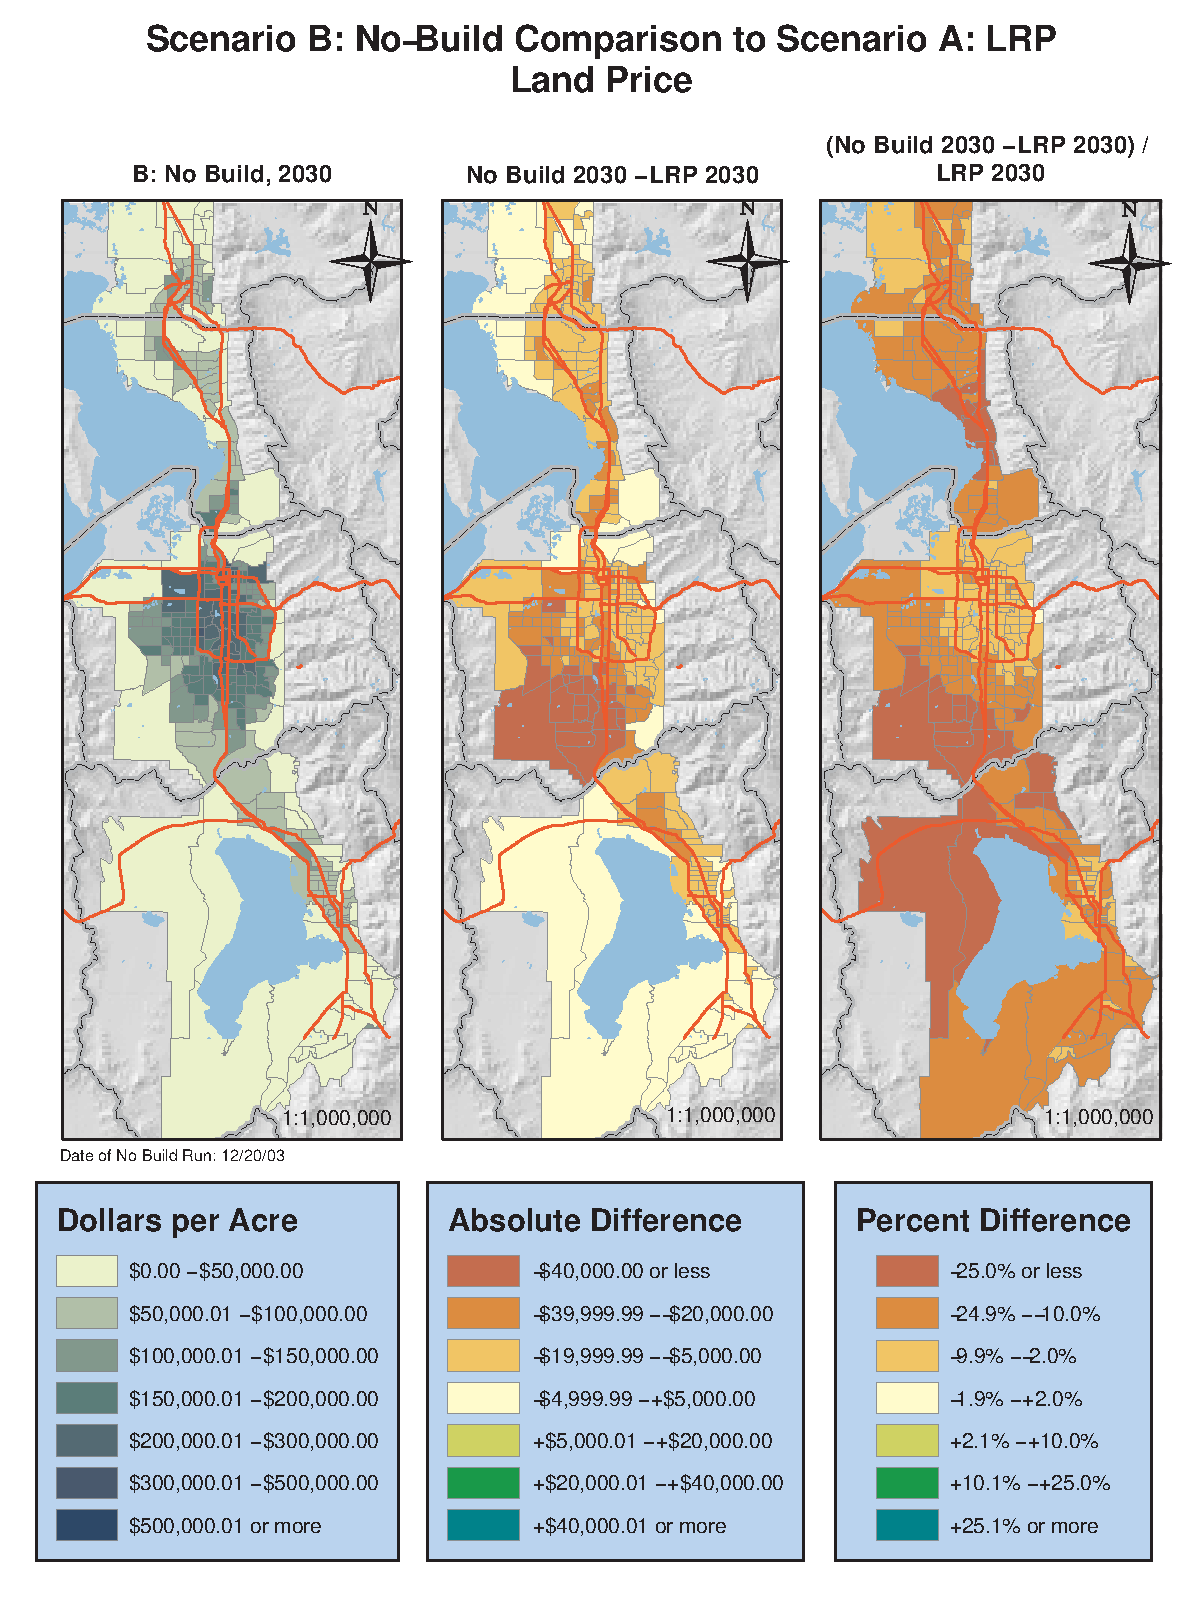
\includegraphics[width=6.0in]{AB_land_price_2030.eps}
%\caption{Comparison of Average Land Price in 2030 between No-Build
%and LRP Scenarios.} \label{fig:AB-land-price}
%\end{figure}
%\clearpage

%\begin{figure}
%\center
%\includegraphics[width=6.0in]{AB_residential_units_2030.eps}
%\caption{Comparison of Housing Density in 2030 between No-Build and
%LRP Scenarios.} \label{fig:AB-res-units}
%\end{figure}
%\clearpage


%\section{Informative Tables}
%\section{Result Tables}
%\input result_tables

\end{document}
